\section{Pianificazione}
Sulla base delle scadenze fissate in §1.6, la ripartizione delle attività di progetto avviene tramite:
\begin{itemize}
\item \textbf{Analisi};
\item \textbf{Consolidamento requisiti};
\item \textbf{Progettazione e codifica per la Technology Baseline};
\item \textbf{Progettazione di dettaglio e codifica};
\item \textbf{Validazione e collaudo}.
\end{itemize}  

\subsection{Analisi}
\textit{Periodo: da 2020-03-16 a 2020-04-13} \\
Durante questo periodo il \textit{TeamAFK} si occuperà principalmente dell’analisi di tutte le informazioni riguardanti il prodotto che deve sviluppare, l’organizzazione delle attività e la suddivisione delle risorse.

\subsubsection{attivi} 
\begin{itemize}
\item \textit{Responsabile di Progetto};
\item \textit{Amministratore};
\item \textit{Analista};
\item \textit{Progettista};
\item \textit{Verificatore}.
\end{itemize}

\subsubsection{Attività}
\begin{itemize}
\item \textbf{Identificazione degli strumenti}: attività rivolta a determinare gli strumenti da utilizzare per le comunicazioni, stesura dei documenti, versionamento, sviluppo e verifica del sistema;
\item \textbf{Norme di Progetto}: sono l'insieme delle regole da seguire per lo svolgimento dei processi e la realizzazione del prodotto. Il documento \textit{Norme di Progetto} è redatto dall'\textit{Amministratore};
\item \textbf{Studio di Fattibilità}: attività svolta dagli \textit{Analisti} con lo scopo di analizzare i capitolati in linea generale per stabilire quale di essi sia una proposta realizzabile. Inoltre è un'attività propedeutica all'\textit{Analisi dei Requisiti};
\item \textbf{Analisi dei Requisiti}: sulla base dell'attività precedente, vengono identificati e definiti i requisiti del sistema. Come per il documento \textit{Studio di Fattibilità}, anche \textit{Analisi dei Requisiti} viene redatto dagli \textit{Analisti};
\item \textbf{Piano di Qualifica}: attività dell'\textit{Amministratore} e del \textit{Progettista} che si occupa di stabilire le metodologie per garantire la qualità del prodotto. In particolar modo la seconda figura si focalizza sulla parte programmatica;
\item \textbf{Piano di Progetto}: il lavoro da svolgere viene suddiviso in compiti, risorse e attività da parte del \textit{Responsabile} che ha anche il compito di calcolare il preventivo di periodo del progetto. Il tutto viene riportato sempre da parte del \textit{Responsabile} nel documento \textit{Piano di Progetto};
\item \textbf{Glossario}: tutti i vocaboli di difficile interpretazione vengono individuati e riportati nel documento \textit{Glossario}.
\end{itemize}

\begin{figure}[H]
\centering
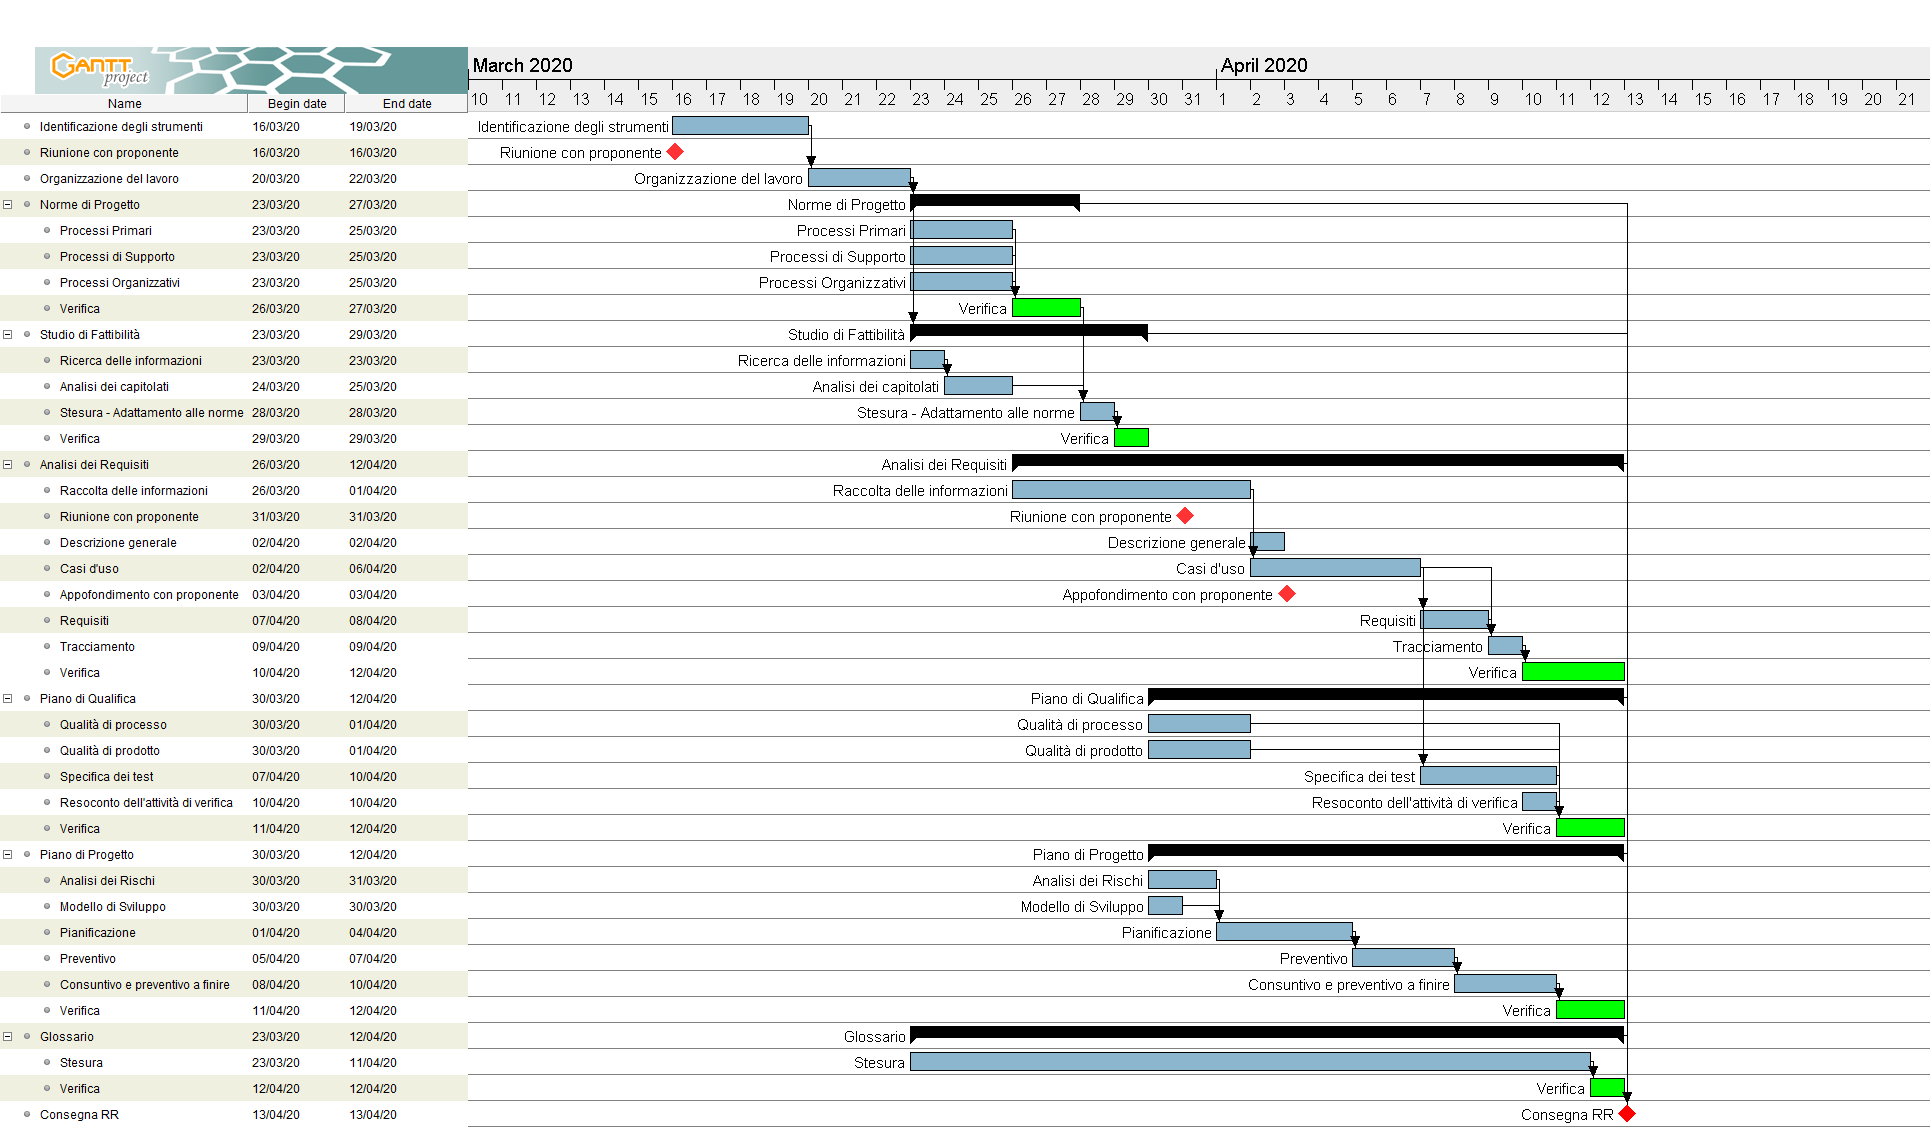
\includegraphics[scale=0.24]{./img/gantt/analisi.png}
\caption{Diagramma di Gantt della fase di Analisi}
\end{figure}

\subsection{Consolidamento dei requisiti}
\textit{Periodo: da 2020-04-14 a 2020-04-20}\\
La fase di consolidamento è così suddivisa:
\begin{itemize}
\item \textbf{Approfondimento personale}: attività intenta a fissare ed approfondire le informazioni riguardanti i requisiti evidenziati nella precedente fase;
\item \textbf{Raccolta informazioni}: raccolta delle informazioni necessarie per la presentazione;
\item \textbf{Stesura presentazione}: preparazione del materiale necessario alla presentazione del 2020-04-20;
\item \textbf{Studio personale}: tempo dedicato ai membri del gruppo, per studiare le informazioni contenute nella presentazione.
\end{itemize}

\begin{figure}[H]
\centering
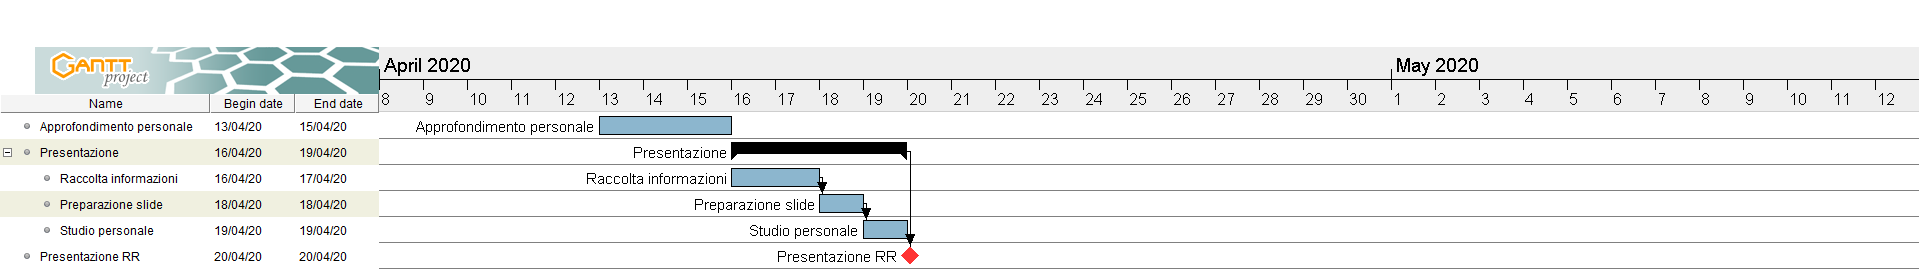
\includegraphics[scale=0.24]{./img/gantt/consolidamento_requisiti.png}
\caption{Diagramma di Gantt della fase di Consolidamento dei requisiti}
\end{figure}

\subsection{Progettazione e codifica per la Technology Baseline}
\textit{Periodo: da 2020-04-21 a 2020-05-11}\\
Questa fase coincide con il giorno successivo alla presentazione del 2020-04-20 e termina con la consegna del materiale per la \textbf{Revisone di Progettazione}.

\subsubsection{Ruoli attivi} \begin{itemize}
\item \textit{Responsabile di Progetto};
\item \textit{Amministratore};
\item \textit{Analista};
\item \textit{Progettista};
\item \textit{Programmatore};
\item \textit{Verificatore}.
\end{itemize}

\subsubsection{Attività}
\begin{itemize}
\item \textbf{Incrementi e verifica dei documenti}: sulla base dei feedback del committente e del proponente, viene migliorato e verificato il materiale del precedente rilascio;
\item \textbf{Progettazione e codifica della Proof of Concept}: vengono identificati i design pattern\glo necessari allo sviluppo del sistema e verranno riportati nell'allegato tecnico insieme al tracciamento dei requisiti. Inoltre viene presentato, al committente e al proponente, un prototipo per mezzo di un repository\glo. In questo periodo saranno implementati solo una parte di requisiti, ovvero quelli che ricoprono le funzionalità del tool di addestramento. La scrittura del codice per lo sviluppo di tali requisiti segue le indicazioni definite nel documento \textit{Norme di Progetto};
\item \textbf{Verifica della Proof of Concept}: vengono testati e verificati tutti gli incrementi sviluppati;
\item \textbf{Preparazione della presentazione}: vengono create le slide da utilizzare per la presentazione della PoC, fissata in data 2020/05/05.
\end{itemize}

\paragraph{Incremento 1}\mbox{} \\ \mbox{} \\ 
\textit{Periodo: da 2020/04/21 a 2020/04/30}\\
L’incremento 1 prevede lo sviluppo e l’implementazione del tool di addestramento, per ottenere il file JSON contenente i predittori. Per sviluppare questo incremento verrà utilizzata la libreria di JS \texttt{JSON.stringify}. \\
Verrà quindi implementata una pagina web che consentirà di: \begin{itemize}
\item caricare il file CSV contenente i dati per l'addestramento;
\item selezionare l'algoritmo di predizione desiderato;
\begin{itemize}
\item nel caso in cui l’utente selezioni un algoritmo incompatibile con il file CSV caricato, sarà mostrato il messaggio di errore "File CSV incompatibile";
\item nel caso in cui l'utente selezioni l'algoritmo senza aver caricato il file CSV, sarà mostrato il messaggio di errore "File CSV non inserito";
\end{itemize}
\item confermare tale algoritmo, per procedere con l'addestramento;
\begin{itemize}
\item l’utente visualizza il messaggio di notifica "Addestramento avvenuto successo", in cui viene notificato che l’addestramento confermato dell’algoritmo selezionato,a partire dai dati di addestramento, è avvenuto correttamente;
\end{itemize}
\item scaricare il file JSON contenente i predittori.
\end{itemize}
Lo sviluppo di questo incremento prevede il soddisfacimento completo dei seguenti requisiti funzionali:
\begin{itemize}
\item Re1F1;
\item Re1F1.1;
\item Re1F1.2;
\item Re1F1.3;
\item Re1F1.6;
\item Re1F9.
\end{itemize}
\paragraph*{Verifica}\mbox{} \\ \mbox{} \\ 
\textit{Periodo: da 2020/05/01 a 2020/05/04}\\
Durante questo periodo verranno testate e verificate tutte le funzionalità di questo incremento. Qualora dovessero presentarsi dei bug\glo, sarà compito dei programmatori risolverli nel più breve tempo possibile.

\paragraph{Incremento 2}\mbox{} \\ \mbox{} \\ 
\textit{Periodo: da 2020/04/21 a 2020/04/30}\\
L’incremento 2 prevede lo sviluppo e l’implementazione dell'algoritmo che permette l'inserimento del file JSON, contenente i predittori, nel plug-in. Verrà usato React in sinergia con gli strumenti di sviluppo di plug-in offerti dalla piattaforma Grafana. \\
Sarà quindi possibile:
\begin{itemize}
	\item selezionare il file json da caricare, presente nel file system;
	\item confermare la selezione.
\end{itemize}
Lo sviluppo di questo incremento prevede il soddisfacimento completo dei seguenti requisiti funzionali:
\begin{itemize}
\item Re1F2;
\item Re1F2.1;
\item Re1F2.2.
\end{itemize}
\paragraph*{Verifica}\mbox{} \\ \mbox{} \\ 
\textit{Periodo: da 2020/05/01 a 2020/05/03}\\
Durante questo periodo verranno testate e verificate tutte le funzionalità di questo incremento. Qualora dovessero presentarsi dei bug, sarà compito dei programmatori risolverli nel più breve tempo possibile.

\paragraph{Incremento 3}\mbox{} \\ \mbox{} \\ 
\textit{Periodo: da 2020/04/21 a 2020/04/30}\\
L’incremento 3 prevede lo sviluppo e l’implementazione dell'algoritmo che permette il collegamento del plug-in ad un flusso di dati. Verrà usato React in sinergia con gli strumenti di sviluppo di plug-in offerti dalla piattaforma Grafana. \\
Sarà quindi possibile:
\begin{itemize}
	\item selezionare i predittori;
	\item selezionare la query legata al flusso dei dati.
\end{itemize}
Lo sviluppo di questo incremento prevede il soddisfacimento completo dei seguenti requisiti funzionali:
\begin{itemize}
\item Re1F3.1;
\item Re1F3.2.
\end{itemize}
\paragraph*{Verifica}\mbox{} \\ \mbox{} \\ 
\textit{Periodo: da 2020/05/01 a 2020/05/03}\\
Durante questo periodo verranno testate e verificate tutte le funzionalità di questo incremento. Qualora dovessero presentarsi dei bug, sarà compito dei programmatori risolverli nel più breve tempo possibile.

\begin{figure}[H]
\centering
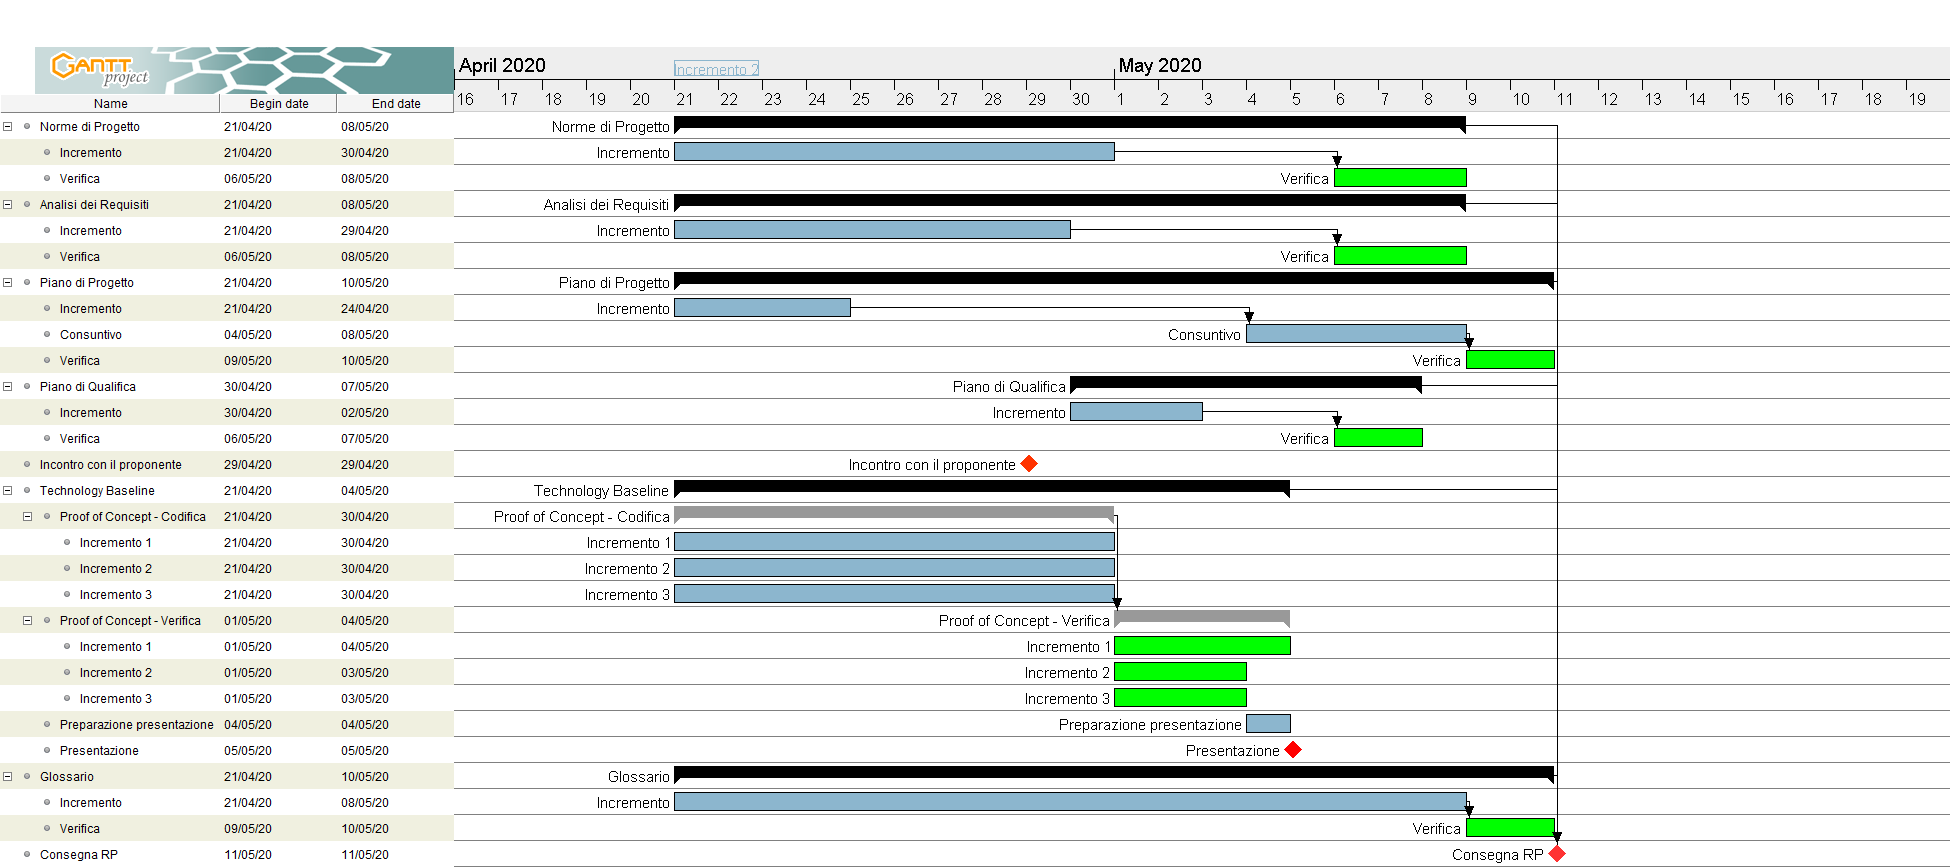
\includegraphics[scale=0.24]{./img/gantt/progettazione_architetturale.png}
\caption{Diagramma di Gantt della fase di Progettazione e codifica per la Technology Baseline}
\end{figure}

\subsection{Progettazine di dettaglio e codifica}
\textit{Periodo: da 2020-05-11 a 2020-06-11}\\
Questa fase è compresa tra il giorno successivo alla presentazione del 2020-05-11 e la consegna della \textit{Revisione di Qualifica}.

\subsubsection{Ruoli attivi} \begin{itemize}
\item \textit{Responsabile di Progetto};
\item \textit{Amministratore};
\item \textit{Analista};
\item \textit{Progettista};
\item \textit{Programmatore};
\item \textit{Verificatore}.
\end{itemize}

\subsubsection{Attività}
\begin{itemize}
\item \textbf{Incrementi e verifica dei documenti}: sulla base dei feedback del committente e del proponente, viene migliorato e verificato il materiale del precedente rilascio;
\item \textbf{Codifica degli incrementi}: 
\item \textbf{Verifica degli incrementi}: 
\item \textbf{Preparazione della presentazione}: vengono create le slide da utilizzare per la presentazione della Product Baseline, fissata in data xxxxxxxxxxxxxxxxxxxxxxxxx.
\end{itemize}

\paragraph{Incremento 4}\mbox{} \\ \mbox{} \\ 
\textit{Periodo: da 2020-05-22 a 2020-05-26}\\
L’incremento 4 prevede il completamento dello sviluppo del tool di addestramento, aggiungendo i messaggi di alert mancanti.\\
Sarà quindi possibile:
\begin{itemize}
	\item visualizzare il messaggio di addestramento avvenuto con successo;
	\item visualizzare l'errore di addestramento non riuscito;
	\item visualizzare l'errore CSV non caricato;
	\item visualizzare l'alert algoritmo non scelto. 
\end{itemize}
Lo sviluppo di questo incremento prevede il soddisfacimento completo dei seguenti requisiti funzionali:
\begin{itemize}
\item Re1F1.4;
\item Re1F1.5;
\item Re1F7;
\item Re1F8.
\end{itemize}
\paragraph*{Verifica}\mbox{} \\ \mbox{} \\ 
\textit{Periodo: da 2020-05-27 a 2020-05-28}\\
Durante questo periodo verranno testate e verificate tutte le funzionalità di questo incremento. Qualora dovessero presentarsi dei bug, sarà compito dei programmatori risolverli nel più breve tempo possibile.

\paragraph{Incremento 5}\mbox{} \\ \mbox{} \\ 
\textit{Periodo: da 2020-05-22 a 2020-05-25}\\
L’incremento 5 prevede il completamento dello sviluppo del caricamento del file json nel plug-in, aggiungendo i messaggi di alert mancanti.\\
Sarà quindi possibile:
\begin{itemize}
	\item visualizzare il messaggio di avvenuto caricamento del file json;
	\item visualizzare l'alert della presenza di un altro json;
	\item visualizzare l'errore di caricamento non avvenuto. 
\end{itemize}
Lo sviluppo di questo incremento prevede il soddisfacimento completo dei seguenti requisiti funzionali:
\begin{itemize}
\item Re1F2.3;
\item Re1F10;
\item Re1F11.
\end{itemize}
\paragraph*{Verifica}\mbox{} \\ \mbox{} \\ 
\textit{Periodo: da 2020-05-26 a 2020-05-27}\\
Durante questo periodo verranno testate e verificate tutte le funzionalità di questo incremento. Qualora dovessero presentarsi dei bug, sarà compito dei programmatori risolverli nel più breve tempo possibile.

\paragraph{Incremento 6}\mbox{} \\ \mbox{} \\ 
\textit{Periodo: da 2020-05-23 a 2020-05-27}\\
L’incremento 6 prevede lo sviluppo del collegamento del predittore. Per poter svolgere questo incremento è necessario l'aver implementato la lettura del file json in quanto è necessario conoscere i predittori contenuti nel file. \\
Sarà quindi possibile:
\begin{itemize}
	\item scegliere uno o più predittori tra quelli disponibili;
	\item selezionare la query associata al flusso di dati;
	\item impostare le soglie di monitoraggio;
	\item confermare le impostazioni di collegamento.
	\item visualizzare le impostazioni precedentemente impostate
\end{itemize}
Lo sviluppo di questo incremento prevede il soddisfacimento completo dei seguenti requisiti funzionali:
\begin{itemize}
\item Re1F3;
\item Re1F3.3;
\item Re1F3.4;
\item Re1F3.6.
\end{itemize}
\paragraph*{Verifica}\mbox{} \\ \mbox{} \\ 
\textit{Periodo: da 2020-05-30 a 2020-05-30}\\
Durante questo periodo verranno testate e verificate tutte le funzionalità di questo incremento. Qualora dovessero presentarsi dei bug, sarà compito dei programmatori risolverli nel più breve tempo possibile.

\paragraph{Incremento 7}\mbox{} \\ \mbox{} \\ 
\textit{Periodo: da 2020-05-28 a 2020-05-29}\\
L’incremento 7 prevede lo sviluppo dei messaggi d'alert o di errore del collegamento del predittore. Per poter svolgere questo incremento è necessario l'aver implementato il collegamento ai predittori, l'impostazione delle soglie e la conferma delle impostazioni. \\
Sarà quindi possibile:
\begin{itemize}
	\item visualizzare il messaggio di conferma di collegamento al flusso dati;
	\item visualizzare l'errore di soglia non valida;
	\item visualizzare l'errore del non collegamento del predittore.
\end{itemize}
Lo sviluppo di questo incremento prevede il soddisfacimento completo dei seguenti requisiti funzionali:
\begin{itemize}
\item Re1F3.5;
\item Re1F12;
\item Re1F13.
\end{itemize}
\paragraph*{Verifica}\mbox{} \\ \mbox{} \\ 
\textit{Periodo: da 2020-05-30 a 2020-05-30}\\
Durante questo periodo verranno testate e verificate tutte le funzionalità di questo incremento. Qualora dovessero presentarsi dei bug, sarà compito dei programmatori risolverli nel più breve tempo possibile.

\paragraph{Incremento 8}\mbox{} \\ \mbox{} \\ 
\textit{Periodo: da 2020-05-28 a 2020-05-30}\\
L’incremento 8 prevede lo sviluppo della funzionalità di modifica del collegamento dei predittori, più precisamente allo scollegamento dei predittori. Per poter svolgere questo incremento è necessario l'aver implementato il collegamento ai predittori. \\
Sarà quindi possibile:
\begin{itemize}
	\item selezionare di modificare i collegamenti;
	\item selezionare di scollegare il predittore;
	\item visualizzare il messaggio di conferma del scollegamento;
	\item selezionare se confermare o annullare lo scollegamento;
	\item visualizzare il messaggio di avvenuto scollegamento.
\end{itemize}
Lo sviluppo di questo incremento prevede il soddisfacimento completo dei seguenti requisiti funzionali:
\begin{itemize}
\item Re1F4;
\item Re1F4.1;
\item Re1F4.2;
\item Re1F4.3;
\item Re1F4.4;
\item Re1F4.5.
\end{itemize}
\paragraph*{Verifica}\mbox{} \\ \mbox{} \\ 
\textit{Periodo: da 2020-05-31 a 2020-05-31}\\
Durante questo periodo verranno testate e verificate tutte le funzionalità di questo incremento. Qualora dovessero presentarsi dei bug, sarà compito dei programmatori risolverli nel più breve tempo possibile.

\paragraph{Incremento 9}\mbox{} \\ \mbox{} \\ 
\textit{Periodo: da 2020-05-28 a 2020-06-01}\\
L’incremento 9 prevede lo sviluppo del calcolo delle previsioni. Per poter svolgere questo incremento è necessario l'aver implementato il collegamento ai predittori e al flusso dati. \\
Sarà quindi possibile:
\begin{itemize}
	\item selezionare la politica temporale della previsione;
	\item avviare il monitoraggio;
	\item interrompere il monitoraggio.
\end{itemize}
Lo sviluppo di questo incremento prevede il soddisfacimento completo dei seguenti requisiti funzionali:
\begin{itemize}
\item Re1F5;
\item Re1F5.1;
\item Re1F5.2;
\item Re1F5.4.
\end{itemize}
\paragraph*{Verifica}\mbox{} \\ \mbox{} \\ 
\textit{Periodo: da 2020-06-01 a 2020-06-03}\\
Durante questo periodo verranno testate e verificate tutte le funzionalità di questo incremento. Qualora dovessero presentarsi dei bug, sarà compito dei programmatori risolverli nel più breve tempo possibile.

\paragraph{Incremento 10}\mbox{} \\ \mbox{} \\ 
\textit{Periodo: da 2020-06-01 a 2020-06-02}\\
L’incremento 10 prevede lo sviluppo dei messaggi di errore, notifica o alert del calcolo delle previsioni. Per poter svolgere questo incremento è necessario l'aver implementato il collegamento dei predittori, la selezione della politica temporale e il calcolo della previsione. \\
Sarà quindi possibile:
\begin{itemize}
	\item visualizzare il messaggio di conferma dell'avvio del monitoraggio;
	\item visualizzare il messaggio di conferma dell'interruzione del monitoraggio;
	\item visualizzare l'errore di nessuna politica temporale inserita;
	\item visualizzare l'errore di nessun predittore selezionato.
\end{itemize}
Lo sviluppo di questo incremento prevede il soddisfacimento completo dei seguenti requisiti funzionali:
\begin{itemize}
\item Re1F5.3;
\item Re1F5.5;
\item Re1F14;
\item Re1F15.
\end{itemize}
\paragraph*{Verifica}\mbox{} \\ \mbox{} \\ 
\textit{Periodo: da 2020-06-03 a 2020-06-03}\\
Durante questo periodo verranno testate e verificate tutte le funzionalità di questo incremento. Qualora dovessero presentarsi dei bug, sarà compito dei programmatori risolverli nel più breve tempo possibile.

\paragraph{Incremento 11}\mbox{} \\ \mbox{} \\ 
\textit{Periodo: da 2020-05-30 a 2020-05-31}\\
L’incremento 11 prevede lo sviluppo del collegamento al database per il salvataggio delle previsioni. Per poter svolgere questo incremento è necessario l'aver implementato il calcolo delle previsioni. \\
Sarà quindi possibile:
\begin{itemize}
	\item selezionare di salvare le previsioni su un database;
	\item visualizzare il messaggio di conferma del collegamento al database.
\end{itemize}
Lo sviluppo di questo incremento prevede il soddisfacimento completo dei seguenti requisiti funzionali:
\begin{itemize}
\item Re1F5.6;
\item Re1F5.7.
\end{itemize}
\paragraph*{Verifica}\mbox{} \\ \mbox{} \\ 
\textit{Periodo: da 2020-06-01 a 2020-06-01}\\
Durante questo periodo verranno testate e verificate tutte le funzionalità di questo incremento. Qualora dovessero presentarsi dei bug, sarà compito dei programmatori risolverli nel più breve tempo possibile.

\paragraph{Incremento 12}\mbox{} \\ \mbox{} \\ 
\textit{Periodo: da 2020-06-01 a 2020-06-03}\\
L’incremento 12 prevede lo sviluppo della visualizzazione delle previsioni attraverso il panel di Grafana. Per poter svolgere questo incremento è necessario l'aver implementato il calcolo della previsione e la selezione delle soglie di monitoraggio. \\
Sarà quindi possibile:
\begin{itemize}
	\item visualizzare le previsioni effettuate, tramite il grafico;
	\item visualizzare un messaggio di alert quando una soglia viene raggiunta dai dati.
\end{itemize}
Lo sviluppo di questo incremento prevede il soddisfacimento completo dei seguenti requisiti funzionali:
\begin{itemize}
\item Re1F6;
\item Re1F6.1;
\item Re1F6.2.
\end{itemize}
\paragraph*{Verifica}\mbox{} \\ \mbox{} \\ 
\textit{Periodo: da 2020-06-04 a 2020-06-05}\\
Durante questo periodo verranno testate e verificate tutte le funzionalità di questo incremento. Qualora dovessero presentarsi dei bug, sarà compito dei programmatori risolverli nel più breve tempo possibile.

\begin{figure}[H]
\centering
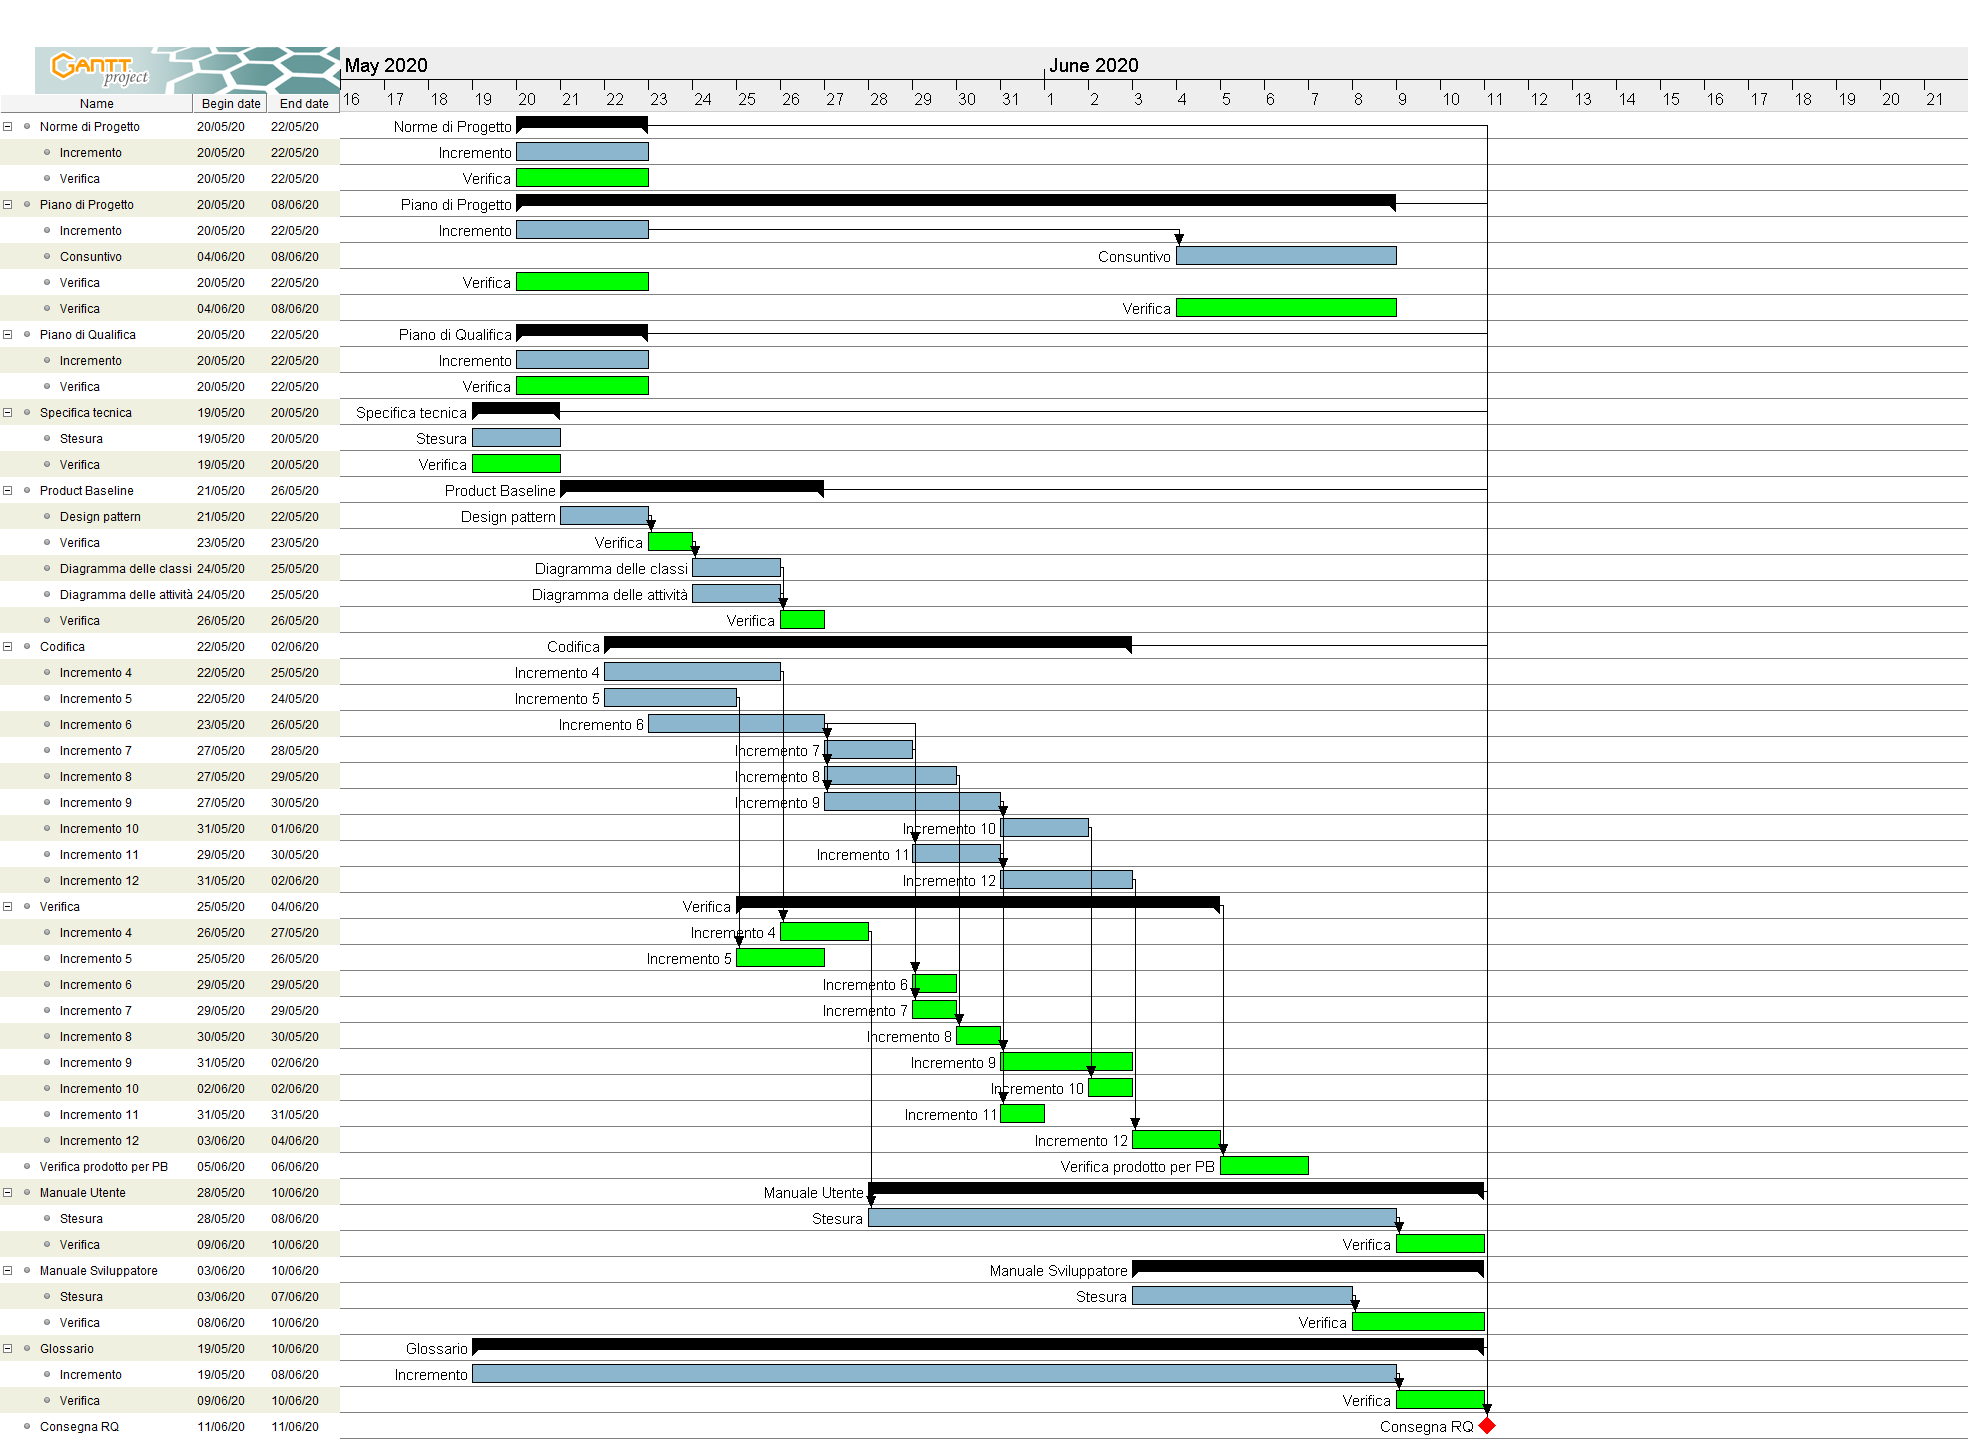
\includegraphics[scale=0.24]{./img/gantt/progettazione_dettaglio_codifica.png}
\caption{Diagramma di Gantt della fase di Progettazione di dettaglio e codifica}
\end{figure}

\subsection{Validazione e collaudo}
\textit{Periodo: da 2020-06-19 a 2020-07-06}\\
La seguente fase inizia il giorno seguente la \textit{Revisione di Qualifica} e termina con la consegna del materiale richiesto per la \textit{Revisione di Avanzamento}.
\begin{itemize}
\item \textbf{Incremento}: nel caso risultasse necessario vengono effettuati miglioramenti sulla base di feedback;
\item \textbf{Validazione e collaudo}: la validazione effettua test sul prodotto, mentre la convalidazione controlla se viene rispettata la coerenza tra il prodotto e le specifiche evidenziate nel documento \textit{Analisi dei Requisiti};
\item \textbf{Manuale Sviluppatore}: viene redatto il documento \textit{Manuale dello Sviluppatore}, il quale conterrà le informazioni necessarie allo sviluppo, mantenimento e manutenzione del prodotto;
\item \textbf{Manuale Utente}: viene redatto il documento \textit{Manuale dell'Utente}, il quale conterrà le informazioni necessarie all'utilizzo del prodotto.
\end{itemize}

\begin{figure}[H]
\centering
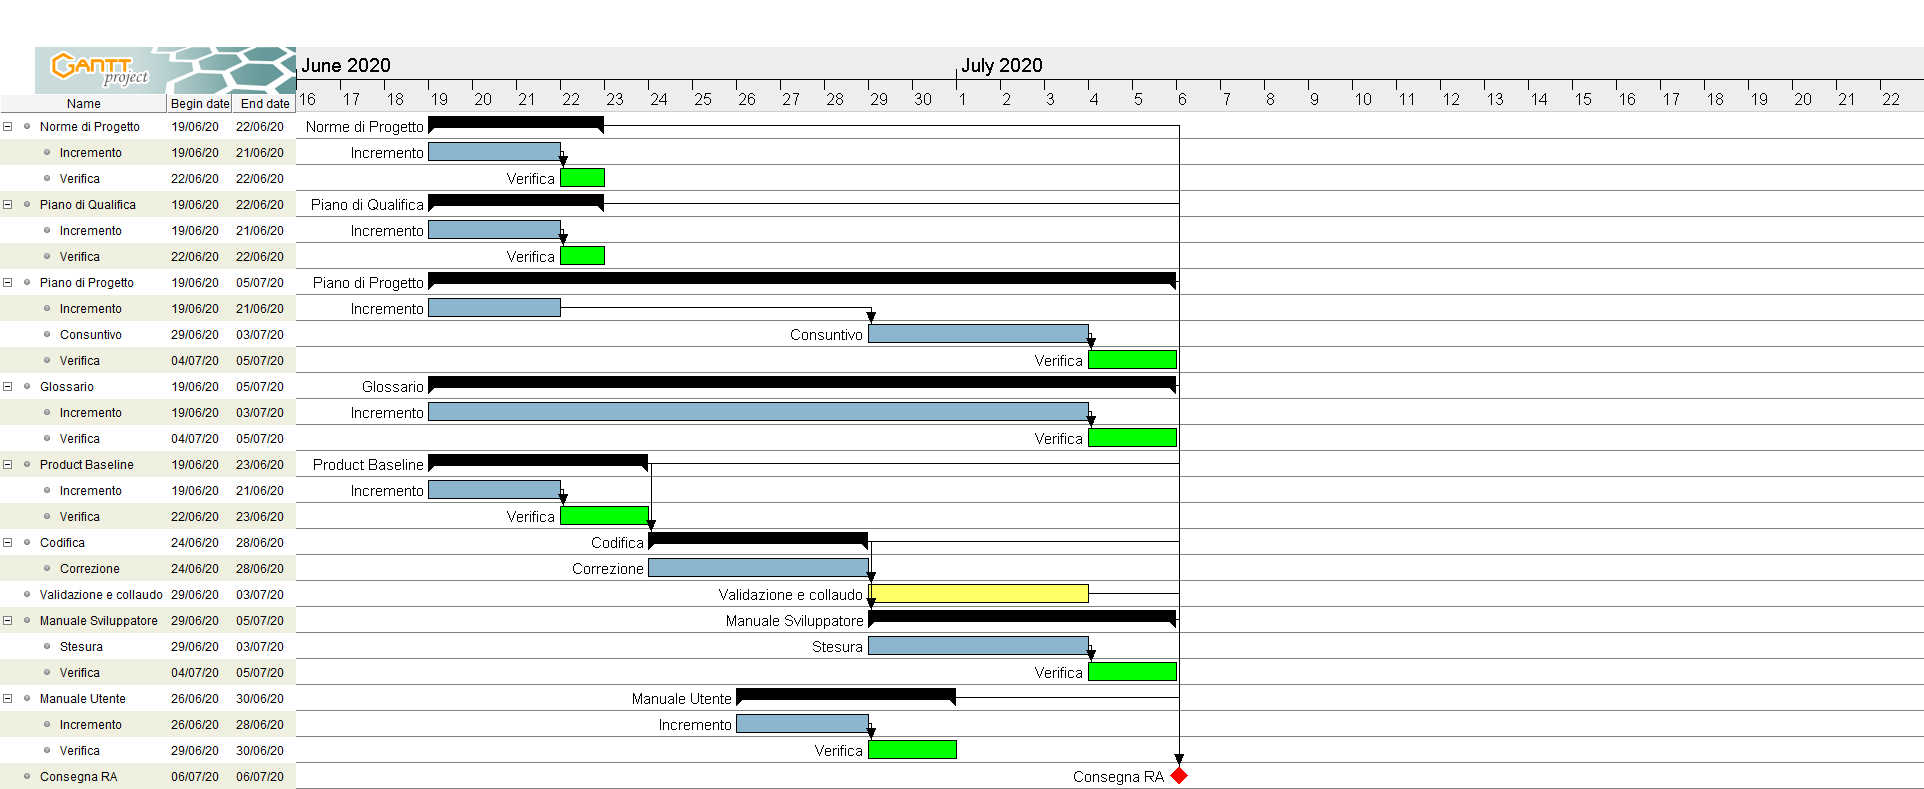
\includegraphics[scale=0.24]{./img/gantt/validazione_collaudo.png}
\caption{Diagramma di Gantt della fase di Validazione e collaudo}
\end{figure}